\section{Auswertung}
\label{sec:Auswertung}

% \begin{figure}
%   \centering
%   \includegraphics{plots/plot.pdf}
%   \caption{Plot.}
%   \label{fig:plot}
% \end{figure}



% \begin{table}
%    % Notation :  {% nicht entfernen ist sehr wichtig sonst Fehler !!
% \parbox{0.48\textwidth}{% %Ermöglicht zwei Tabellen neben einander
%   \centering
%   \sisetup{round-mode = places , round-precision = 0,scientific-notation=fixed, fixed-exponent = 0}
%          %rundet Werte aus Stelle, Stelle = ,  macht einen bestimmten festen exponenten
%   \resizebox{\textwidth}{!}{%  % skaliert zu große Tabellen
%   \begin{tabular}{S@{${}\pm{}$} S} % fügt plus minus Fehler Schreibweise hinzu
%     \toprule
%      $\text{e}_b / \si{\milli\meter}$ &
%      $\text{d}_b /\si{\milli\meter} $ & $\text{f}_b / \si{\milli\meter} $\\
%     \midrule
%     \bottomrule
%   \end{tabular}
%   % }
%   \caption{Tabellenunterschrift}
%   \label{tab:tab}
% }
% % \end{table}
% % \begin{table}
% \parbox{0.48\textwidth}{%
%   \centering
%   \sisetup{round-mode = places , round-precision = 0,scientific-notation=fixed, fixed-exponent = 0}
%   % \resizebox{\textwidth}{!}{%
%   \begin{tabular}{S@{${}\pm{}$} S}
%     \toprule
%      $\text{e}_b / \si{\milli\meter}$ &
%      $\text{d}_b /\si{\milli\meter} $ & $\text{f}_b / \si{\milli\meter} $\\
%     \midrule
%     \bottomrule
%   \end{tabular}
%   % }
%   \caption{Tabellenunterschrift}
%   \label{tab:tab}
% }
% \end{table}
\subsection{Bestimmung der maximalen Kraftflussdichte des mag. Feldes}
\label{sec:BFeld}
Zur Bestimmung der maximalen Kraftflussdichte, wird zu erst die Kraftflussdichte in ein
Diagramm gegen die z-Position aufgetragen und dann mit einer Ausgleichskurve approximiert.
Die Ausgleichskurve wurde mit nicht-linearer Ausgleichsrechnung unter Zurhilfenahme von
\cite{scipy} und folgender Gaußfunktion bestimmt:
\begin{equation*}
	f(z)= \frac{A}{\sqrt{2\pi\sigma}}\cdot\exp\left(-\frac{1}{2} \left(\frac{z}{\sigma} \right) ^2 \right)
\end{equation*}
Daraus ergibt sich, dass $A= \SI{0.0096(4)}{\tesla\meter}$ und $\sigma = \SI{0.0084(4)}{\meter}$
betragen muss. An der Position der Probe ist die Kraftflussdichte maximal, also bei
$z =0$, folglich ergibt sich, dass  die maximale Kraftflussdichte $f(0) = \SI{0.45(2)}{\tesla}$
beträgt. Das zuvor erwähnte Diagramm ist in der Abbildung \ref{fig:BFeld} zusehen, alle Werte
dazu sind in der Tabelle \ref{tab:BFeld} dargestellt.
 \begin{figure}
   \centering
   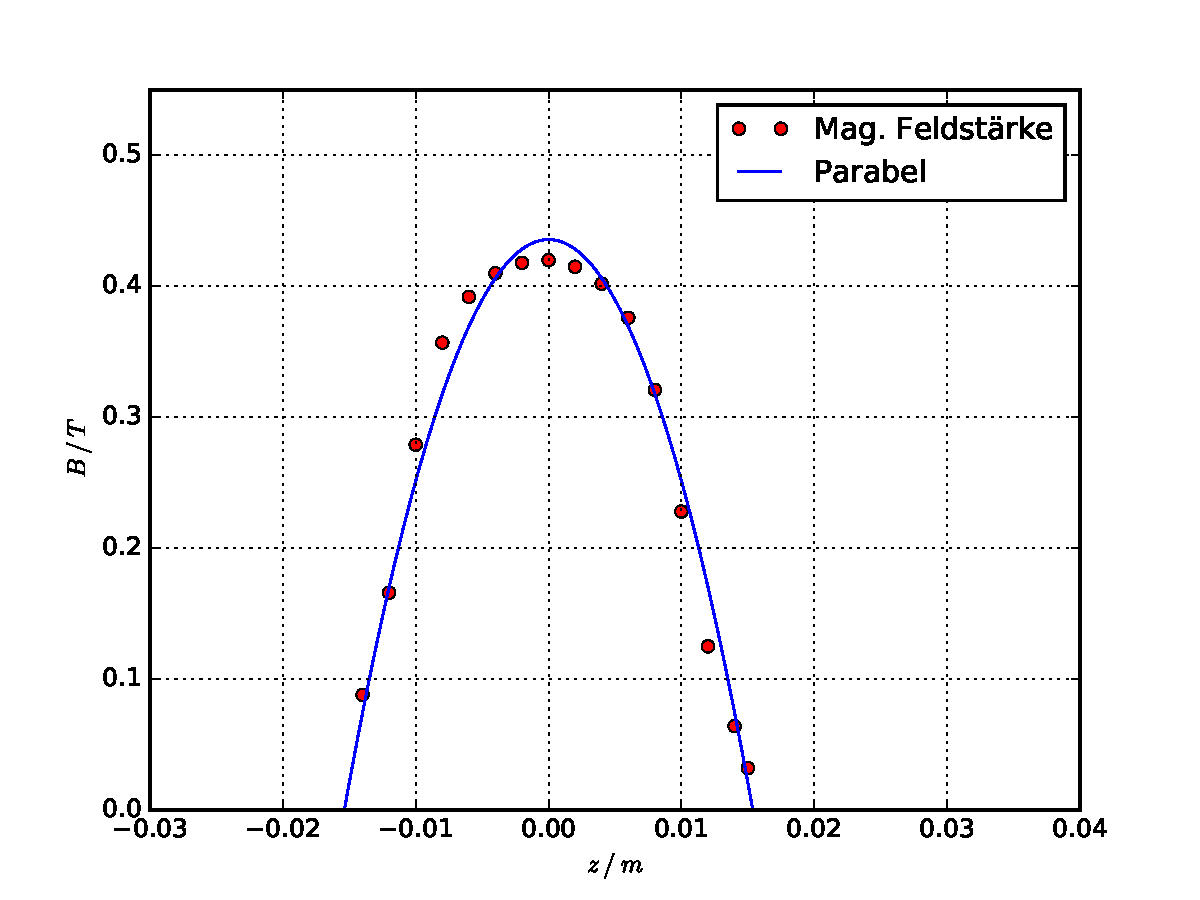
\includegraphics[height= 7cm]{plots/BFeld.pdf}
   \caption{Magnetische Feldstärke parallel zum Strahlengang. Die Probe liegt im Zentrum, hier bei Null. Der Verlauf der Feldstärke wurde mit einer Gaußfunktion approximiert.}
   \label{fig:BFeld}
 \end{figure}

  \begin{table}
   \centering
   \sisetup{round-mode = places , round-precision = 3,scientific-notation=fixed, fixed-exponent = 0}
   \begin{tabular}{S S}
     \toprule
      $\text{Feldstärke\;} B /\si{\tesla} $ & $z \text{-Position} / \si{\meter} $\\
     \midrule
       8.799999999999999489e-02 & -1.400000000000000029e-02\\
       1.660000000000000087e-01 & -1.200000000000000025e-02\\
       2.790000000000000258e-01 & -1.000000000000000021e-02\\
       3.569999999999999840e-01 & -8.000000000000000167e-03\\
       3.920000000000000151e-01 & -6.000000000000000125e-03\\
       4.100000000000000311e-01 & -4.000000000000000083e-03\\
       4.179999999999999827e-01 & -2.000000000000000042e-03\\
       4.199999999999999845e-01 & 0.000000000000000000e+00\\
       4.150000000000000355e-01 & 2.000000000000000042e-03\\
       4.020000000000000240e-01 & 4.000000000000000083e-03\\
       3.760000000000000009e-01 & 6.000000000000000125e-03\\
       3.210000000000000075e-01 & 8.000000000000000167e-03\\
       2.280000000000000082e-01 & 1.000000000000000021e-02\\
       1.250000000000000000e-01 & 1.200000000000000025e-02\\
       6.400000000000000133e-02 & 1.400000000000000029e-02\\
       3.200000000000000067e-02 & 1.499999999999999944e-02\\
     \bottomrule
   \end{tabular}
   \caption{Werte zur Bestimmung der maximalen Kraftflussdichte.}
   \label{tab:BFeld}
  \end{table}

\subsection{Faraday-Rotation an n-dotiertem und hochreinem GaAs}
Zuerst wurden die längennormierten Winkel der Faraday-Rotation gegen die quadrierte Wellenlänge
aufgetragen, dies ist in der Abbildung \ref{fig:Vgl} zusehen.

\begin{figure}
  \centering
  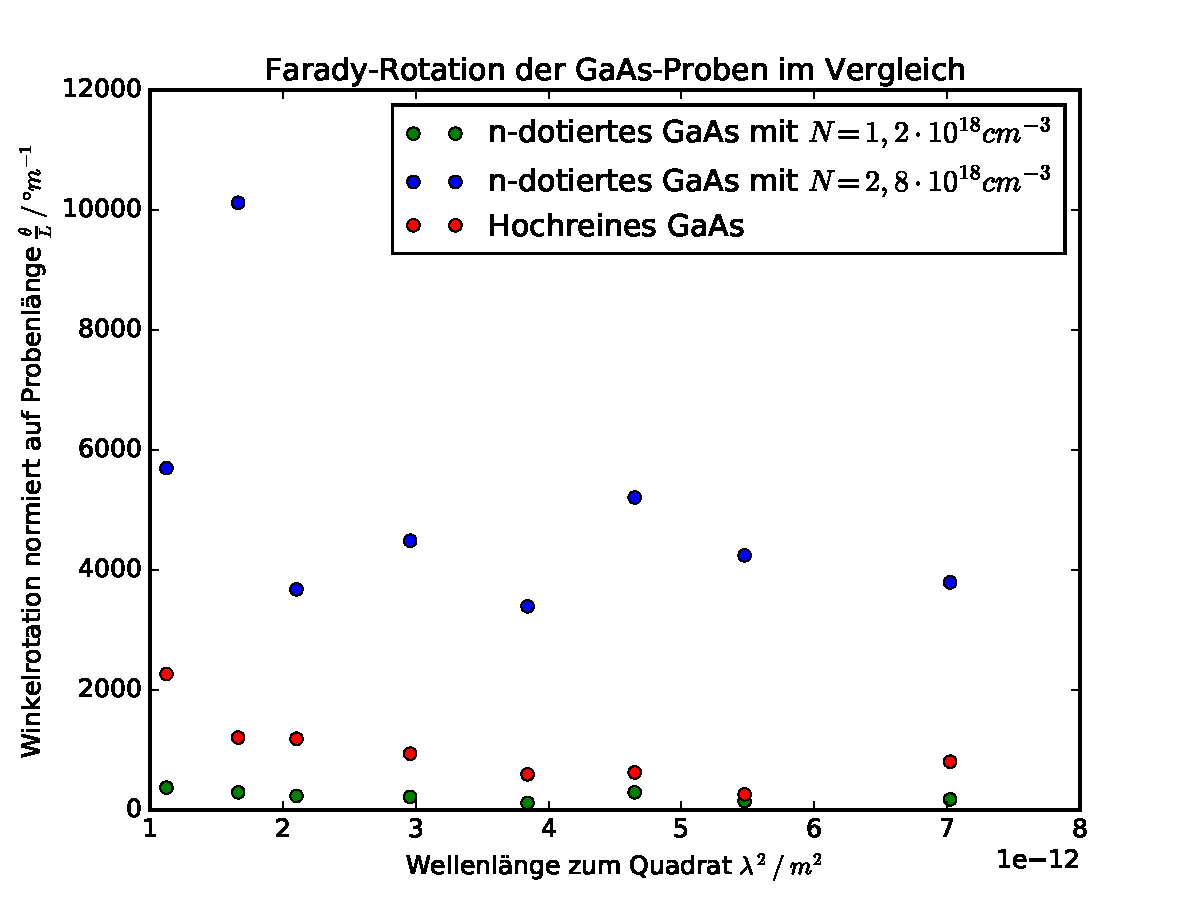
\includegraphics[height=7cm]{plots/GaAsimVgl.pdf}
  \caption{Die Längennormierte Farady-Rotation aller GaAs-Proben im Vergleich.}
  \label{fig:Vgl}
\end{figure}

\subsection{Bestimmung der effektiven Masse}
Zur Bestimmung der effektiven Masse der Elektronen in GaAs wurden zuerst
die Differenz der längennomierten Faraday-Rotationen zwischen der hochreinen
Probe und den zwei n-dotierten gegen die quadrierte Wellenlänge aufgetragen.
Das ist in der Abbildung \ref{fig:Delta} festgehalten.
Dann wurde mit linearer Ausgleichsrechnung eine Ausgleichgerade durch den Nullpunkt bestimmt.
Dazu wurde die einfache Geradengleichung
\begin{equation*}
 f\left(x\right) = a \cdot x +b
\end{equation*}
verwendet. Daraus ergibt sich für Differenz mit der $N = \SI{2.8e18}{\per\cubic\centi\meter}$
n-dotierten Probe $a = \SI{9.1(26)e14}{\per\meter}$ und für die
$N = \SI{1.2e18}{\per\cubic\centi\meter}$
n-dotierten Probe $a= \SI{3.3(15)e14}{\per\meter}$. Aus der Gleichung \eqref{eq:Winkelfrei}
folgt dann für die effektive Masse:

\begin{equation}
m^* = \sqrt{\frac{\symup{e}_0 ^3 N B}{8\pi^2 \epsilon_0 \symup{c}^3 n a}} \qquad .
\end{equation}

Hier bei ist $\symup{e}_0$ die Elementarladung, $\symup{c}$ die Lichtgeschwindigkeit
und $\epsilon_0$ die elektrische Feldkonstante, alle
physikalischen Konstanten wurden zur Berechnung aus \cite{scipy} importiert. Die Größe $N$
bezeichnet die freien Ladungsträger pro Kubikzentimeter in den n-dotierten Proben, $B$ bezeichnet
die magnetische Feldstärke die in Kapitel \ref{sec:BFeld} bestimmt wurde.
Die Größe $n$ ist der Brechungsindex für GaAs, dieser wurde mit 3,3543 für eine Wellenlänge
von \SI{1771.14}{\nano\meter} angenommen, da der Mittelwert der von uns benutzten Wellenlängen bei
\SI{1.8}{\micro\meter} liegt.
Der Brechungsindex wurde aus Quelle \cite{BIndex} entnommen.
Dann ergibt sich für die effektive Masse für die
$N = \SI{2.8e18}{\per\cubic\centi\meter}$
n-dotierten Probe $m_1 ^* = \SI{1.0(15)e-6}{\per\meter}\cdot m_e$ und
für die $N = \SI{1.2e18}{\per\cubic\centi\meter}$
n-dotierten Probe $m_2 ^* = \SI{1.1(26)e-6}{\per\meter}\cdot m_e$, hier bezeichnet $m_e$ die
Elektronenmasse importiert aus \cite{scipy}. Der Fehler der effektiven Massen wurde wie folgt
bestimmt:
\begin{equation*}
\Delta m^*= \sqrt{\left(\frac{\partial m^*\left(a,B\right)}{\partial a} \Delta a\right)^2 + \left(\frac{\partial m^*\left(a,B\right)}{\partial B} \Delta B\right)^2} \qquad .
\end{equation*}
Alle Werte dazu sind in den Tabellen \ref{tab:HGaAstab},
\ref{tab:1.nGaAstab} und \ref{tab:2.nGaAstab} dargestellt.
\begin{figure}
  \centering
  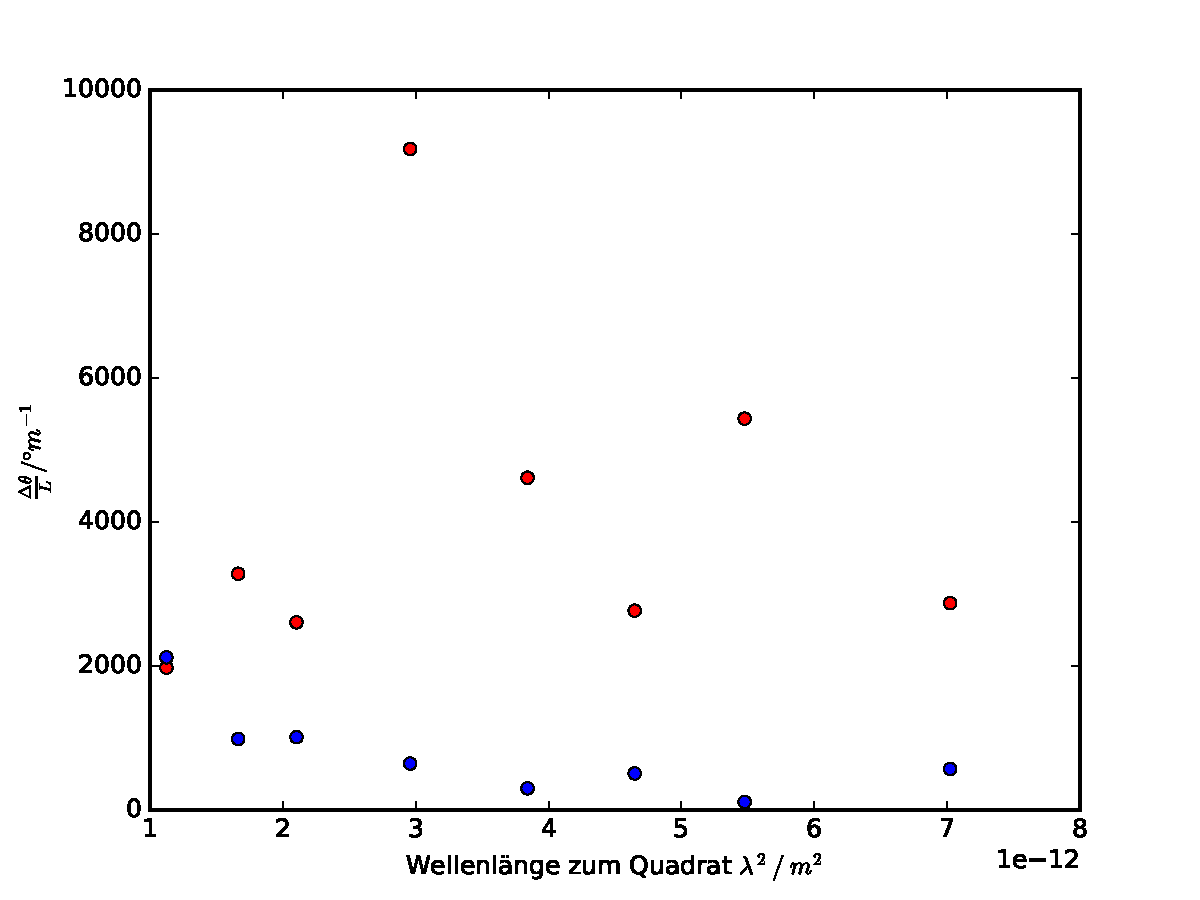
\includegraphics[height=7cm]{plots/DeltaTheta.pdf}
  \caption{Differenzen der längennormierten Faraday-Rotationen zwischen der hochreinen und den
zwei n-dotierten Proben, aufgetragen gegen die quadrierte Wellenlänge.}
  \label{fig:Delta}
\end{figure}

\begin{table}
  \centering
  \sisetup{round-mode = places , round-precision = 2}
  \begin{tabular}{S[scientific-notation=fixed, fixed-exponent =-6] S[scientific-notation=fixed, fixed-exponent = 0] S[scientific-notation=fixed, fixed-exponent = 0]}
    \toprule
    $\text{Wellenlänge} \lambda / \si{\meter}$ & $ \text{Faraday-Rotation\;} \theta / \si{\degree}$ &$ \text{Längenormierte Faraday-Rotation\;} \frac{\theta}{d=\SI{5.11}{\milli\meter}} / \si{\degree\per\meter}$ \\
    \midrule
    1.959999999999999869e-06&3.033333333333331439e+00&5.936073059360726347e+02\\
    1.719999999999999837e-06&4.799999999999997158e+00&9.393346379647742879e+02\\
    2.649999999999999615e-06&4.116666666666660035e+00&8.056099151989549227e+02\\
    2.339999999999999619e-06&1.333333333333328596e+00&2.609262883235476238e+02\\
    1.060000000000000016e-06&1.158333333333332860e+01&2.266797129810827300e+03\\
    1.449999999999999881e-06&6.066666666666662877e+00&1.187214611872145269e+03\\
    1.289999999999999931e-06&6.166666666666671404e+00&1.206784083496412904e+03\\
    2.156000000000000195e-06&3.200000000000002842e+00&6.262230919765171393e+02\\
    \bottomrule
  \end{tabular}
  \caption{Werte des hochreinen GaAs im Überblick.}
  \label{tab:HGaAstab}
%}
\end{table}
\begin{table}
%\parbox{0.48\textwidth}{%
  \centering
  \sisetup{round-mode = places , round-precision = 2}
  \begin{tabular}{S[scientific-notation=fixed, fixed-exponent =-6] S[scientific-notation=fixed, fixed-exponent = 0] S[scientific-notation=fixed, fixed-exponent = 0]}
    \toprule
	    $\text{Wellenlänge} \lambda / \si{\meter}$ & $ \text{Faraday-Rotation\;} \theta / \si{\degree}$ &$ \text{Längenormierte Faraday-Rotation\;} \frac{\theta}{d=\SI{1.296}{\milli\meter}} / \si{\degree\per\meter}$ \\
    \midrule
    2.156000000000000195e-06 & 6.750000000000000000e+00 & 5.208333333333333030e+03\\
    1.289999999999999931e-06 & 1.311666666666666003e+01 & 1.012088477366254665e+04\\
    1.449999999999999881e-06 & 4.766666666666665719e+00 & 3.677983539094649132e+03\\
    1.060000000000000016e-06 & 7.383333333333339965e+00 & 5.697016460905354506e+03\\
    2.339999999999999619e-06 & 5.500000000000000000e+00 & 4.243827160493827250e+03\\
    2.649999999999999615e-06 & 4.916666666666657193e+00 & 3.793724279835383641e+03\\
    1.719999999999999837e-06 & 5.816666666666677088e+00 & 4.488168724279843445e+03\\
    1.959999999999999869e-06 & 4.400000000000005684e+00 & 3.395061728395065984e+03\\
    \bottomrule
  \end{tabular}
  \caption{Werte des \texorpdfstring{$N = \SI{2.8e18}{\per\cubic\centi\meter}$}{math} n-dotierten GaAs im Überblick.}
  \label{tab:1.nGaAstab}
%}
\end{table}
\begin{table}
 \centering
 \sisetup{round-mode = places , round-precision = 2}
 \begin{tabular}{S[scientific-notation=fixed, fixed-exponent =-6] S[scientific-notation=fixed, fixed-exponent = 0] S[scientific-notation=fixed, fixed-exponent = 0]}
   \toprule
   $\text{Wellenlänge} \lambda / \si{\meter}$ & $ \text{Faraday-Rotation\;} \theta / \si{\degree}$ &$ \text{Längenormierte Faraday-Rotation\;} \frac{\theta}{d=\SI{1.36}{\milli\meter}} / \si{\degree\per\meter}$ \\

   \midrule
    2.156000000000000195e-06 & 4.000000000000000000e+00 & 2.941176470588235361e+02\\
    1.289999999999999931e-06 & 4.000000000000000000e+00 & 2.941176470588235361e+02\\
    1.449999999999999881e-06 & 3.199999999999988631e+00 & 2.352941176470579592e+02\\
    1.060000000000000016e-06 & 5.066666666666662877e+00 & 3.725490196078428085e+02\\
    2.339999999999999619e-06 & 2.000000000000000000e+00 & 1.470588235294117680e+02\\
    2.649999999999999615e-06 & 2.400000000000005684e+00 & 1.764705882352945139e+02\\
    1.719999999999999837e-06 & 2.983333333333334281e+00 & 2.193627450980392837e+02\\
    1.959999999999999869e-06 & 1.616666666666660035e+00 & 1.188725490196073480e+02\\
   \bottomrule
 \end{tabular}
  \caption{Werte des \texorpdfstring{$N = \SI{1.2e18}{\per\cubic\centi\meter}$}{math} n-dotierten GaAs im Überblick.}
  \label{tab:2.nGaAstab}
\end{table}
